%-------------------------------------------------------------------------------
%  \author Jan P Buchmann <jan.buchmann@sydney.edu.au>
%  \copyright 2018 The University of Sydney
%  \description
%-------------------------------------------------------------------------------
\begin{figure}
  \begin{lrbox}{\mylistingbox}%
      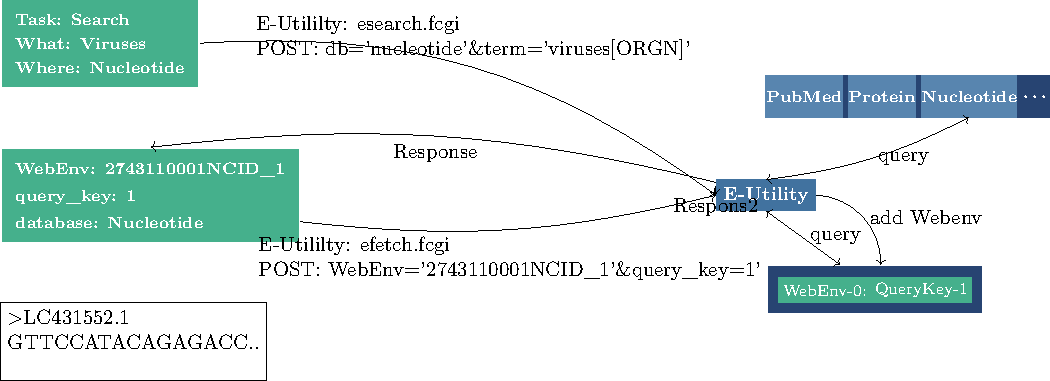
\includegraphics{workflows/eutils_simple_fig.pdf}
  \end{lrbox}%
  \subfloat[Example of searching the Entrez databases using \entrezpy esearcher.
            The nucleotide Entrez database is queried for UIDs  with the
            term 'biomo trna' in their property field. The found UIDs are
            printed to the standard output using the default EsearcherAnalyzer.]
            {\usebox{\mylistingbox}\label{subfig:esearch}}%
%next  subfigure
\hfill
\begin{lrbox}{\mylistingboxII}%
      \begin{bash}
esearch -db gene -query "tp53[preferred symbol] AND human[orgn]"  \|
elink -target protein  | esummary  \ |
xtract -pattern DocumentSummary -element Caption SourceDb
\end{bash}
  \end{lrbox}%
  \subfloat[Entrez Direct example to fetch the 'caption' and 'source database'
            information for sequences in the protein database linked from
            results in the gene database]{\usebox{\mylistingboxII}\label{subfig:edirect}}%
%next  subfigure
\hfill
  \begin{lrbox}{\mylistingboxIII}%
      \begin{python}
import wally.wally

p = {'db':'gene', 'term':'tp53[preferred symbol] AND human[organism]'}
w = wally.wally.Wally(email)
px = w.new_pipeline()
qid = px.add_search(parameter=p)
qid = px.add_link(parameter={'db' : 'protein'}, dependency=qid)
qid = px.add_summary(dependency=qid)
analyzer = w.run(px)
for i in analyzer.result.summaries:
  print(analyzer.result.summaries[i].get('caption'),
        analyzer.result.summaries[i].get('sourcedb')))
\end{python}%
  \end{lrbox}%
  \subfloat[\entrezpy Wally example reproducing Figure~\ref{subfig:edirect}]
  {\usebox{\mylistingboxIII}\label{subfig:wally}}%
  \caption{\entrezpy usage examples. Figure~\ref{subfig:edirect} depicts a query
           using the Entrez Direct tool. Figure~\ref{subfig:esearch} shows
           the usage for a single E-Utility function, here ESearch.
           Figure~\ref{subfig:wally} shows the same query as
           Figure~\ref{subfig:edirect} using the Wally class from \entrezpy. The
           email parameter in the \entrezpy examples indicates the email of the
           developer as required by NCBI
  \label{fig:entrezpy_examples}}
\end{figure}
